%% bare_jrnl.tex
%% V1.4b
%% 2015/08/26
%% by Michael Shell
%% see http://www.michaelshell.org/
%% for current contact information.
%%
%% This is a skeleton file demonstrating the use of IEEEtran.cls
%% (requires IEEEtran.cls version 1.8b or later) with an IEEE
%% journal paper.
%%
%% Support sites:
%% http://www.michaelshell.org/tex/ieeetran/
%% http://www.ctan.org/pkg/ieeetran
%% and
%% http://www.ieee.org/

%%*************************************************************************
%% Legal Notice:
%% This code is offered as-is without any warranty either expressed or
%% implied; without even the implied warranty of MERCHANTABILITY or
%% FITNESS FOR A PARTICULAR PURPOSE! 
%% User assumes all risk.
%% In no event shall the IEEE or any contributor to this code be liable for
%% any damages or losses, including, but not limited to, incidental,
%% consequential, or any other damages, resulting from the use or misuse
%% of any information contained here.
%%
%% All comments are the opinions of their respective authors and are not
%% necessarily endorsed by the IEEE.
%%
%% This work is distributed under the LaTeX Project Public License (LPPL)
%% ( http://www.latex-project.org/ ) version 1.3, and may be freely used,
%% distributed and modified. A copy of the LPPL, version 1.3, is included
%% in the base LaTeX documentation of all distributions of LaTeX released
%% 2003/12/01 or later.
%% Retain all contribution notices and credits.
%% ** Modified files should be clearly indicated as such, including  **
%% ** renaming them and changing author support contact information. **
%%*************************************************************************


% *** Authors should verify (and, if needed, correct) their LaTeX system  ***
% *** with the testflow diagnostic prior to trusting their LaTeX platform ***
% *** with production work. The IEEE's font choices and paper sizes can   ***
% *** trigger bugs that do not appear when using other class files.       ***                          ***
% The testflow support page is at:
% http://www.michaelshell.org/tex/testflow/



\documentclass[journal]{IEEEtran}
%
% If IEEEtran.cls has not been installed into the LaTeX system files,
% manually specify the path to it like:
% \documentclass[journal]{../sty/IEEEtran}





% Some very useful LaTeX packages include:
% (uncomment the ones you want to load)


% *** MISC UTILITY PACKAGES ***
%
%\usepackage{ifpdf}
% Heiko Oberdiek's ifpdf.sty is very useful if you need conditional
% compilation based on whether the output is pdf or dvi.
% usage:
% \ifpdf
%   % pdf code
% \else
%   % dvi code
% \fi
% The latest version of ifpdf.sty can be obtained from:
% http://www.ctan.org/pkg/ifpdf
% Also, note that IEEEtran.cls V1.7 and later provides a builtin
% \ifCLASSINFOpdf conditional that works the same way.
% When switching from latex to pdflatex and vice-versa, the compiler may
% have to be run twice to clear warning/error messages.






% *** CITATION PACKAGES ***
%
%\usepackage{cite}
% cite.sty was written by Donald Arseneau
% V1.6 and later of IEEEtran pre-defines the format of the cite.sty package
% \cite{} output to follow that of the IEEE. Loading the cite package will
% result in citation numbers being automatically sorted and properly
% "compressed/ranged". e.g., [1], [9], [2], [7], [5], [6] without using
% cite.sty will become [1], [2], [5]--[7], [9] using cite.sty. cite.sty's
% \cite will automatically add leading space, if needed. Use cite.sty's
% noadjust option (cite.sty V3.8 and later) if you want to turn this off
% such as if a citation ever needs to be enclosed in parenthesis.
% cite.sty is already installed on most LaTeX systems. Be sure and use
% version 5.0 (2009-03-20) and later if using hyperref.sty.
% The latest version can be obtained at:
% http://www.ctan.org/pkg/cite
% The documentation is contained in the cite.sty file itself.






% *** GRAPHICS RELATED PACKAGES ***
%
\ifCLASSINFOpdf
  \usepackage[pdftex]{graphicx}
  % declare the path(s) where your graphic files are
  % \graphicspath{{../pdf/}{../jpeg/}}
  % and their extensions so you won't have to specify these with
  % every instance of \includegraphics
  % \DeclareGraphicsExtensions{.pdf,.jpeg,.png}
\else
  % or other class option (dvipsone, dvipdf, if not using dvips). graphicx
  % will default to the driver specified in the system graphics.cfg if no
  % driver is specified.
  % \usepackage[dvips]{graphicx}
  % declare the path(s) where your graphic files are
  % \graphicspath{{../eps/}}
  % and their extensions so you won't have to specify these with
  % every instance of \includegraphics
  % \DeclareGraphicsExtensions{.eps}
\fi
\usepackage{tikz}
\usepackage[edges]{forest}
% graphicx was written by David Carlisle and Sebastian Rahtz. It is
% required if you want graphics, photos, etc. graphicx.sty is already
% installed on most LaTeX systems. The latest version and documentation
% can be obtained at: 
% http://www.ctan.org/pkg/graphicx
% Another good source of documentation is "Using Imported Graphics in
% LaTeX2e" by Keith Reckdahl which can be found at:
% http://www.ctan.org/pkg/epslatex
%
% latex, and pdflatex in dvi mode, support graphics in encapsulated
% postscript (.eps) format. pdflatex in pdf mode supports graphics
% in .pdf, .jpeg, .png and .mps (metapost) formats. Users should ensure
% that all non-photo figures use a vector format (.eps, .pdf, .mps) and
% not a bitmapped formats (.jpeg, .png). The IEEE frowns on bitmapped formats
% which can result in "jaggedy"/blurry rendering of lines and letters as
% well as large increases in file sizes.
%
% You can find documentation about the pdfTeX application at:
% http://www.tug.org/applications/pdftex





% *** MATH PACKAGES ***
%
%\usepackage{amsmath}
% A popular package from the American Mathematical Society that provides
% many useful and powerful commands for dealing with mathematics.
%
% Note that the amsmath package sets \interdisplaylinepenalty to 10000
% thus preventing page breaks from occurring within multiline equations. Use:
%\interdisplaylinepenalty=2500
% after loading amsmath to restore such page breaks as IEEEtran.cls normally
% does. amsmath.sty is already installed on most LaTeX systems. The latest
% version and documentation can be obtained at:
% http://www.ctan.org/pkg/amsmath





% *** SPECIALIZED LIST PACKAGES ***
%
%\usepackage{algorithmic}
% algorithmic.sty was written by Peter Williams and Rogerio Brito.
% This package provides an algorithmic environment fo describing algorithms.
% You can use the algorithmic environment in-text or within a figure
% environment to provide for a floating algorithm. Do NOT use the algorithm
% floating environment provided by algorithm.sty (by the same authors) or
% algorithm2e.sty (by Christophe Fiorio) as the IEEE does not use dedicated
% algorithm float types and packages that provide these will not provide
% correct IEEE style captions. The latest version and documentation of
% algorithmic.sty can be obtained at:
% http://www.ctan.org/pkg/algorithms
% Also of interest may be the (relatively newer and more customizable)
% algorithmicx.sty package by Szasz Janos:
% http://www.ctan.org/pkg/algorithmicx




% *** ALIGNMENT PACKAGES ***
%
%\usepackage{array}
% Frank Mittelbach's and David Carlisle's array.sty patches and improves
% the standard LaTeX2e array and tabular environments to provide better
% appearance and additional user controls. As the default LaTeX2e table
% generation code is lacking to the point of almost being broken with
% respect to the quality of the end results, all users are strongly
% advised to use an enhanced (at the very least that provided by array.sty)
% set of table tools. array.sty is already installed on most systems. The
% latest version and documentation can be obtained at:
% http://www.ctan.org/pkg/array


% IEEEtran contains the IEEEeqnarray family of commands that can be used to
% generate multiline equations as well as matrices, tables, etc., of high
% quality.




% *** SUBFIGURE PACKAGES ***
%\ifCLASSOPTIONcompsoc
%  \usepackage[caption=false,font=normalsize,labelfont=sf,textfont=sf]{subfig}
%\else
%  \usepackage[caption=false,font=footnotesize]{subfig}
%\fi
% subfig.sty, written by Steven Douglas Cochran, is the modern replacement
% for subfigure.sty, the latter of which is no longer maintained and is
% incompatible with some LaTeX packages including fixltx2e. However,
% subfig.sty requires and automatically loads Axel Sommerfeldt's caption.sty
% which will override IEEEtran.cls' handling of captions and this will result
% in non-IEEE style figure/table captions. To prevent this problem, be sure
% and invoke subfig.sty's "caption=false" package option (available since
% subfig.sty version 1.3, 2005/06/28) as this is will preserve IEEEtran.cls
% handling of captions.
% Note that the Computer Society format requires a larger sans serif font
% than the serif footnote size font used in traditional IEEE formatting
% and thus the need to invoke different subfig.sty package options depending
% on whether compsoc mode has been enabled.
%
% The latest version and documentation of subfig.sty can be obtained at:
% http://www.ctan.org/pkg/subfig




% *** FLOAT PACKAGES ***
%
%\usepackage{fixltx2e}
% fixltx2e, the successor to the earlier fix2col.sty, was written by
% Frank Mittelbach and David Carlisle. This package corrects a few problems
% in the LaTeX2e kernel, the most notable of which is that in current
% LaTeX2e releases, the ordering of single and double column floats is not
% guaranteed to be preserved. Thus, an unpatched LaTeX2e can allow a
% single column figure to be placed prior to an earlier double column
% figure.
% Be aware that LaTeX2e kernels dated 2015 and later have fixltx2e.sty's
% corrections already built into the system in which case a warning will
% be issued if an attempt is made to load fixltx2e.sty as it is no longer
% needed.
% The latest version and documentation can be found at:
% http://www.ctan.org/pkg/fixltx2e


%\usepackage{stfloats}
% stfloats.sty was written by Sigitas Tolusis. This package gives LaTeX2e
% the ability to do double column floats at the bottom of the page as well
% as the top. (e.g., "\begin{figure*}[!b]" is not normally possible in
% LaTeX2e). It also provides a command:
%\fnbelowfloat
% to enable the placement of footnotes below bottom floats (the standard
% LaTeX2e kernel puts them above bottom floats). This is an invasive package
% which rewrites many portions of the LaTeX2e float routines. It may not work
% with other packages that modify the LaTeX2e float routines. The latest
% version and documentation can be obtained at:
% http://www.ctan.org/pkg/stfloats
% Do not use the stfloats baselinefloat ability as the IEEE does not allow
% \baselineskip to stretch. Authors submitting work to the IEEE should note
% that the IEEE rarely uses double column equations and that authors should try
% to avoid such use. Do not be tempted to use the cuted.sty or midfloat.sty
% packages (also by Sigitas Tolusis) as the IEEE does not format its papers in
% such ways.
% Do not attempt to use stfloats with fixltx2e as they are incompatible.
% Instead, use Morten Hogholm'a dblfloatfix which combines the features
% of both fixltx2e and stfloats:
%
% \usepackage{dblfloatfix}
% The latest version can be found at:
% http://www.ctan.org/pkg/dblfloatfix




%\ifCLASSOPTIONcaptionsoff
%  \usepackage[nomarkers]{endfloat}
% \let\MYoriglatexcaption\caption
% \renewcommand{\caption}[2][\relax]{\MYoriglatexcaption[#2]{#2}}
%\fi
% endfloat.sty was written by James Darrell McCauley, Jeff Goldberg and 
% Axel Sommerfeldt. This package may be useful when used in conjunction with 
% IEEEtran.cls'  captionsoff option. Some IEEE journals/societies require that
% submissions have lists of figures/tables at the end of the paper and that
% figures/tables without any captions are placed on a page by themselves at
% the end of the document. If needed, the draftcls IEEEtran class option or
% \CLASSINPUTbaselinestretch interface can be used to increase the line
% spacing as well. Be sure and use the nomarkers option of endfloat to
% prevent endfloat from "marking" where the figures would have been placed
% in the text. The two hack lines of code above are a slight modification of
% that suggested by in the endfloat docs (section 8.4.1) to ensure that
% the full captions always appear in the list of figures/tables - even if
% the user used the short optional argument of \caption[]{}.
% IEEE papers do not typically make use of \caption[]'s optional argument,
% so this should not be an issue. A similar trick can be used to disable
% captions of packages such as subfig.sty that lack options to turn off
% the subcaptions:
% For subfig.sty:
% \let\MYorigsubfloat\subfloat
% \renewcommand{\subfloat}[2][\relax]{\MYorigsubfloat[]{#2}}
% However, the above trick will not work if both optional arguments of
% the \subfloat command are used. Furthermore, there needs to be a
% description of each subfigure *somewhere* and endfloat does not add
% subfigure captions to its list of figures. Thus, the best approach is to
% avoid the use of subfigure captions (many IEEE journals avoid them anyway)
% and instead reference/explain all the subfigures within the main caption.
% The latest version of endfloat.sty and its documentation can obtained at:
% http://www.ctan.org/pkg/endfloat
%
% The IEEEtran \ifCLASSOPTIONcaptionsoff conditional can also be used
% later in the document, say, to conditionally put the References on a 
% page by themselves.




% *** PDF, URL AND HYPERLINK PACKAGES ***
%
%\usepackage{url}
% url.sty was written by Donald Arseneau. It provides better support for
% handling and breaking URLs. url.sty is already installed on most LaTeX
% systems. The latest version and documentation can be obtained at:
% http://www.ctan.org/pkg/url
% Basically, \url{my_url_here}.




% *** Do not adjust lengths that control margins, column widths, etc. ***
% *** Do not use packages that alter fonts (such as pslatex).         ***
% There should be no need to do such things with IEEEtran.cls V1.6 and later.
% (Unless specifically asked to do so by the journal or conference you plan
% to submit to, of course. )


% correct bad hyphenation here
\hyphenation{op-tical net-works semi-conduc-tor}


\begin{document}
%
% paper title
% Titles are generally capitalized except for words such as a, an, and, as,
% at, but, by, for, in, nor, of, on, or, the, to and up, which are usually
% not capitalized unless they are the first or last word of the title.
% Linebreaks \\ can be used within to get better formatting as desired.
% Do not put math or special symbols in the title.
\title{Target-driven Genetic Programming of\\ Music Patterns with TidalCycles}
%
%
% author names and IEEE memberships
% note positions of commas and nonbreaking spaces ( ~ ) LaTeX will not break
% a structure at a ~ so this keeps an author's name from being broken across
% two lines.
% use \thanks{} to gain access to the first footnote area
% a separate \thanks must be used for each paragraph as LaTeX2e's \thanks
% was not built to handle multiple paragraphs
%

\author{Federico~Rubbi,
        Jie~Chen,
        Stefano~Camposilvan,
        and~Valeria~Miroslava~Mayora~Barcenas% <-this % stops a space
\thanks{M. Shell was with the Department
of Electrical and Computer Engineering, Georgia Institute of Technology, Atlanta,
GA, 30332 USA e-mail: (see http://www.michaelshell.org/contact.html).}% <-this % stops a space
\thanks{J. Doe and J. Doe are with Anonymous University.}% <-this % stops a space
\thanks{Manuscript received April 19, 2005; revised August 26, 2015.}}

% note the % following the last \IEEEmembership and also \thanks - 
% these prevent an unwanted space from occurring between the last author name
% and the end of the author line. i.e., if you had this:
% 
% \author{....lastname \thanks{...} \thanks{...} }
%                     ^------------^------------^----Do not want these spaces!
%
% a space would be appended to the last name and could cause every name on that
% line to be shifted left slightly. This is one of those "LaTeX things". For
% instance, "\textbf{A} \textbf{B}" will typeset as "A B" not "AB". To get
% "AB" then you have to do: "\textbf{A}\textbf{B}"
% \thanks is no different in this regard, so shield the last } of each \thanks
% that ends a line with a % and do not let a space in before the next \thanks.
% Spaces after \IEEEmembership other than the last one are OK (and needed) as
% you are supposed to have spaces between the names. For what it is worth,
% this is a minor point as most people would not even notice if the said evil
% space somehow managed to creep in.



% The paper headers
\markboth{BIO-INSPIRED ARTIFICIAL INTELLIGENCE COURSE PROJECT REPORT, 2025-2026}%
{Target-driven Genetic Programming of Music Patterns with TidalCycles}
% The only time the second header will appear is for the odd numbered pages
% after the title page when using the twoside option.
% 
% *** Note that you probably will NOT want to include the author's ***
% *** name in the headers of peer review papers.                   ***
% You can use \ifCLASSOPTIONpeerreview for conditional compilation here if
% you desire.




% If you want to put a publisher's ID mark on the page you can do it like
% this:
%\IEEEpubid{0000--0000/00\$00.00~\copyright~2015 IEEE}
% Remember, if you use this you must call \IEEEpubidadjcol in the second
% column for its text to clear the IEEEpubid mark.



% use for special paper notices
%\IEEEspecialpapernotice{(Invited Paper)}




% make the title area
\maketitle







% For peer review papers, you can put extra information on the cover
% page as needed:
% \ifCLASSOPTIONpeerreview
% \begin{center} \bfseries EDICS Category: 3-BBND \end{center}
% \fi
%
% For peerreview papers, this IEEEtran command inserts a page break and
% creates the second title. It will be ignored for other modes.
\IEEEpeerreviewmaketitle



\section{Introduction}
\IEEEPARstart{T}{his} project investigates how genetic programming can be used to
automatically discover musical patterns in the live coding language
TidalCycles such that their rendered audio approximates a given target
recording.
Rather than evolving music ``in the abstract'', we adopt a
target-driven perspective: the goal is to search directly in the space of
TidalCycles programs for patterns whose audio is as close as possible to a
fixed example clip.

To make this feasible, we represent individuals as typed expression trees
generated from a grammar that encodes a subset of the Tidal pattern
language, ensuring that all genomes correspond to syntactically valid
code.
Each candidate pattern is rendered to audio via a TidalCycles/SuperDirt
backend and evaluated with a composite fitness function that measures
similarity to the target along multiple musical dimensions, including
timbre, harmony, rhythm, dynamics and tempo.

In summary, the report covers: (i) a grammar-based genome
representation for genetic programming over TidalCycles patterns;
(ii) a multi-feature audio similarity fitness tailored to this domain; and
(iii) an empirical study of how these design choices influence the
evolution of patterns toward a fixed audio target.
The remainder of the report first reviews related work on evolutionary
music and live coding, then details the proposed method, experimental
setup and results, and concludes with a discussion of limitations and
future directions.

\section{Related Work}
Evolutionary and other bio-inspired algorithms have been applied to music
generation since the early 1990s, from genetic algorithms for
computer-assisted composition and jazz improvisation~\cite{Horner1991_GA_Music,Biles1994_GenJam}
to grammar-based methods that evolve complete musical
structures~\cite{McCormack1996_GrammarMusic,Puente2002_GrammaticalMusic,Reddin2009_ElevatedPitch,Loughran2015_TonalityGE}.
These systems typically operate in a symbolic domain (scores, MIDI or
domain-specific languages) and use evolutionary search to explore musical
spaces subject to style or constraint rules, rather than to approximate a
specific external recording.

Designing fitness functions that capture musical goals is a central
challenge.
Feature-based evolutionary music systems~\cite{Papadopoulos1999_AISurvey}
often define targets for musical descriptors and reward individuals that
match these targets, for example using statistical properties such as
Zipfian pitch and rhythm distributions~\cite{Manaris2007_ZipfMusic} or
weighted combinations of melodic and rhythmic
features~\cite{Ozcan2008_ImprovisedMusicGA}.
Other work uses music-theoretic constraints and tension profiles to steer
generation toward a desired style or structure~\cite{Herremans2016_Morpheus}.
In the audio domain, evolutionary techniques have been used to match
low-level sound targets, such as evolving FM synthesizer parameters to
imitate a reference timbre via spectral distance
measures~\cite{Horner1993_FMGA}, or evolving in learned latent spaces
defined by autoencoders~\cite{McArthur2021_AutoencoderGA}.
However, there are still relatively few systems that evolve symbolic music
directly against a concrete audio recording using an expressively rich
similarity objective.

Live coding environments such as TidalCycles~\cite{McLean2010_Tidal}
enable musicians to write and transform musical patterns as code in
real time.
Several authors have explored integrating evolutionary algorithms into
live coding, for example by evolving Tidal pattern variations that can be
selected during performance~\cite{Hickinbotham2016_LiveCodingEA} or by
using genetic algorithms to generate and manipulate musical code in
improvisational contexts~\cite{Dasari2020_LiveCodingGA}.
These approaches typically employ interactive or novelty-driven fitness
and focus on exploratory creativity.
In contrast, our work brings a target-driven perspective to the live
coding domain: we evolve TidalCycles pattern code so that its rendered
audio approaches a fixed reference clip, using a fully automatic
multi-feature audio similarity fitness and no human-in-the-loop
evaluation.

\section{Problem Statement and Approach}
The problem we address can be stated as follows: given a fixed target audio
clip of limited duration, we seek a TidalCycles pattern whose rendered audio
matches the target as closely as possible according to a set of perceptually
motivated similarity measures.
The search space is the set of syntactically valid TidalCycles pattern
expressions expressible within a bounded context-free grammar; the objective is to
maximize a scalar fitness that aggregates multiple audio-feature similarities
between the rendered candidate and the target.

Our approach decomposes this problem into three main components.
First, a grammar-based genome representation encodes TidalCycles patterns as
typed expression trees, together with a set of mutation and crossover
operators that explore the space while preserving syntactic validity.
Second, a backend layer interfaces with TidalCycles and SuperDirt to render
each candidate pattern to audio under controlled conditions.
Third, a fitness evaluation module extracts timbral, harmonic, rhythmic,
dynamic and tempo descriptors from both candidate and target audio and
combines them into a single similarity score used by the genetic programming
loop.
By iteratively sampling, evaluating and selecting genomes, the system
evolves pattern code whose audio output progressively approaches the target.

\section{Method}
\label{sec:method}

\subsection{System Overview}
At a high level, the system implements a standard evolutionary loop
specialized for TidalCycles patterns.
An initial population of genomes is created by sampling random pattern
expression trees from the Tidal grammar within a bounded depth.
In each generation, the algorithm converts every genome to TidalCycles code,
renders the corresponding audio, evaluates its fitness against the target,
and then applies selection and variation operators to form the next
population.

\begin{figure}[!t]
  \centering
  % \includegraphics[width=\linewidth]{figures/architecture.pdf}
  \caption{High-level architecture of the target-driven TidalCycles evolution
  system, showing the flow from genomes to code, audio rendering, fitness
  evaluation and evolutionary search.}
  \label{fig:architecture}
\end{figure}

The implementation is organized into three main modules.
The \emph{genome} and \emph{generator} modules provide the pattern-tree
representation and the mutation/crossover operators.
The \emph{backend} module manages a GHCi/TidalCycles/SuperDirt session,
allowing the system to send pattern code and record audio snippets under
controlled conditions.
The \emph{fitness evaluation} module computes perceptually motivated
similarity measures between the rendered candidate audio and the target, and
aggregates them into a scalar fitness used by the genetic programming loop.

\subsection{Pattern Representation and Genetic Operators}

\subsubsection{Grammar and Pattern Trees}
To ensure that all evolved individuals are syntactically valid TidalCycles
patterns, we base our representation on a family of grammar modules written
in Lark's EBNF-inspired format and compiled to an LALR(1) parser~\cite{Shinan2020_Lark}.
These grammars define typed pattern expressions (e.g., notes, numbers,
booleans, time values) by combining terminal symbols (tokens) with
non-terminal production rules.
Non-terminals such as \texttt{pattern\_note}, \texttt{pattern\_int} and
\texttt{pattern\_time} encode the structure of different pattern types,
while terminals represent note names, sample identifiers, numeric literals
and operator tokens.
For example, the top-level control-pattern rule in one of our grammar
modules is written as:
{\fontsize{8.59}{10.87}\selectfont
\begin{verbatim}
?control_pattern: cp_playable_term 
                  (cp_infix_op cp_playable_term)*
\end{verbatim}
}
which states (in Lark's EBNF-like syntax) that a \texttt{control\_pattern}
consists of one or more \texttt{cp\_playable\_term} expressions combined by
an infix operator layer \texttt{cp\_infix\_op}. More specifically, the import-closed grammar used in our experiments spans 13 Lark
modules and 239 production rules.
As shown by static analysis tools, the symbol dependency graph consists 45 distinct terminal
symbols and 193 non-terminals.
The terminals cover typed scalar tokens (integers, floating-point numbers,
booleans, strings and the special \emph{silence} symbol), explicit operator
tokens for arithmetic, pattern combination and time shifting, and curated
finite string domains that restrict sample, scale, parameter and bus names to
values that exist in our SuperDirt setup.
The non-terminals can be organized into three broad families:
(i) a control-pattern layer that ensures every sentence contains at least one
sound-producing head (e.g., \texttt{cp\_sound\_atom}, rhythmic combinators
such as \texttt{cp\_euclid\_playable}, higher-order applicators like
\texttt{cp\_applied\_playable});
(ii) six typed subgrammars for time, integers, doubles, strings, notes and
booleans, each providing literals, list constructors, time-based
concatenations and prefix/transform operators for its sort;
and (iii) auxiliary helper rules for lists, time pairs and domain-specific
scalar arguments.
While the full grammar graph produced by our visualization tool is too large
to include as a figure, these statistics illustrate that the search space is
defined by a fairly rich yet strongly structured fragment of the Tidal
pattern language.

Genomes are instantiated as \emph{pattern trees}, where each node
corresponds to a Tidal operator (e.g., \texttt{sound}, \texttt{fast},
\texttt{struct}, \texttt{stack}) or a terminal value.
The \texttt{PatternTree} and underlying node classes provide basic
operations such as computing depth and size, iterating over nodes, and
reconstructing the corresponding Tidal expression.
Because trees are generated and transformed in accordance with the grammar,
genetic operators cannot produce malformed code.
Figure~\ref{fig:pattern-tree} shows a small example tree for the pattern
\texttt{fast 2 (stack[s("bd"), s("sn")])}, highlighting how timing transforms,
list combinators and sound atoms are combined hierarchically.

\begin{figure}[!t]
  \centering
  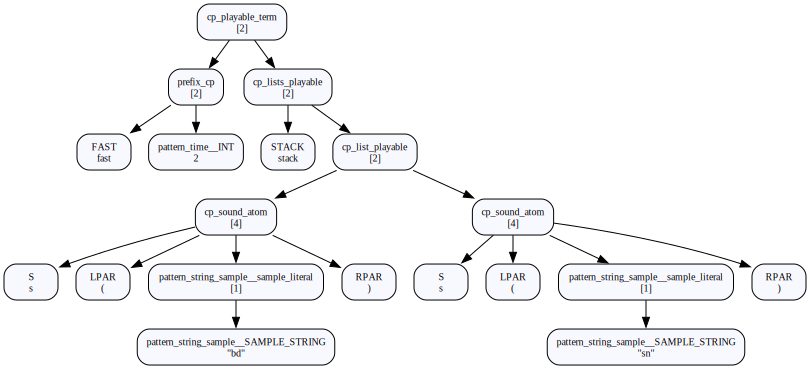
\includegraphics[width=\columnwidth]{../data/figures/pattern_tree.pdf}
  \caption{Example pattern tree for the TidalCycles expression
  \texttt{fast 2 (stack[s("bd"), s("sn")])}, illustrating the hierarchical
  combination of a timing transform (\texttt{fast}), a list combinator
  (\texttt{stack}) and two sound-producing atoms (\texttt{sound} ``bd'',
  \texttt{sound} ``sn'').}
  \label{fig:pattern-tree}
\end{figure}

\subsubsection{Mutation and Crossover}
Variation is implemented through a suite of mutation operators and a
tree-based crossover.
Rather than mutating raw strings, each operator transforms the pattern tree
in a way that corresponds to a meaningful musical edit.
The available mutations can be grouped into a few categories:
\begin{itemize}
  \item \emph{Structural mutations}: operators such as \texttt{append},
        \texttt{truncate} and \texttt{struct} modify the overall shape or
        duration of a pattern by adding or removing segments or changing
        structural masks.
  \item \emph{Rhythmic transformations}: mutations like
        \texttt{euclid} (Euclidean rhythms), \texttt{striate} (time
        slicing) and \texttt{speed} alter the rhythmic subdivision and
        temporal density of events.
  \item \emph{Layering and texture}: \texttt{stack\_wrap},
        \texttt{stack\_enrich} and \texttt{overlay\_wrap} introduce or
        modify layers of concurrent patterns, enriching the texture.
  \item \emph{Pitch and timbre}: \texttt{note\_wrap}, \texttt{scale\_wrap}
        and terminal substitutions change pitch collections, note values or
        sound identifiers while keeping the surrounding structure intact.
\end{itemize}

At each mutation step, the system samples a node (or small subtree) and
applies one of these operators with a configurable probability.
If an operator does not change the tree (e.g.\ due to boundary conditions),
the original genome is retained to avoid unnecessary fitness evaluations.

Crossover operates by identifying nodes with matching operators in two
parent trees and swapping the corresponding subtrees.
Because matching is done on operator type and the trees respect the
underlying grammar, the resulting offspring remain syntactically valid
Tidal patterns.
Selection is performed via tournament selection with elitism: the best
individuals of each generation are carried over unchanged, while the rest of
the population is filled by offspring produced by crossover and mutation.

\subsection{Fitness Evaluation}

Evaluating fitness requires turning each genome into an audio signal and
comparing it with the target.
First, the pattern tree is converted to a TidalCycles expression using a
code-generation function that recursively translates nodes into textual
Tidal code.
This code is then sent to the Tidal backend, which plays the pattern on a
dedicated stream and records a fixed-duration audio clip using SuperDirt.

Given the rendered candidate audio and the target clip, the fitness
evaluation module extracts several standard music-information-retrieval
features using the \texttt{librosa} Python library~\cite{McFee2015_librosa}.
We compute:
\begin{itemize}
  \item Mel-frequency cepstral coefficients (MFCCs) as a proxy for timbral
        similarity;
  \item chroma features to capture harmonic content;
  \item onset-strength envelopes to describe rhythmic patterns;
  \item FFT magnitude spectra and RMS energy curves for spectral shape and
        dynamics;
  \item an estimate of the tempo (in BPM) and a coarse pitch contour.
\end{itemize}
For each feature type, we measure similarity between candidate and target
using frame-wise or vector cosine similarity, after truncating both signals
to a common length.

Finally, these partial similarities are aggregated into a single scalar
fitness by a weighted sum, with higher weights assigned to features deemed
more relevant to the task (e.g.\ timbre and harmony).
The resulting score lies in $[0,1]$ and is maximized by the evolutionary
search.
This design allows us to incorporate multiple musical aspects without
requiring a fully learned embedding or human feedback, while still
providing a quantitative objective that can drive genetic programming over
TidalCycles patterns.


% An example of a floating figure using the graphicx package.
% Note that \label must occur AFTER (or within) \caption.
% For figures, \caption should occur after the \includegraphics.
% Note that IEEEtran v1.7 and later has special internal code that
% is designed to preserve the operation of \label within \caption
% even when the captionsoff option is in effect. However, because
% of issues like this, it may be the safest practice to put all your
% \label just after \caption rather than within \caption{}.
%
% Reminder: the "draftcls" or "draftclsnofoot", not "draft", class
% option should be used if it is desired that the figures are to be
% displayed while in draft mode.
%
%\begin{figure}[!t]
%\centering
%\includegraphics[width=2.5in]{myfigure}
% where an .eps filename suffix will be assumed under latex, 
% and a .pdf suffix will be assumed for pdflatex; or what has been declared
% via \DeclareGraphicsExtensions.
%\caption{Simulation results for the network.}
%\label{fig_sim}
%\end{figure}

% Note that the IEEE typically puts floats only at the top, even when this
% results in a large percentage of a column being occupied by floats.


% An example of a double column floating figure using two subfigures.
% (The subfig.sty package must be loaded for this to work.)
% The subfigure \label commands are set within each subfloat command,
% and the \label for the overall figure must come after \caption.
% \hfil is used as a separator to get equal spacing.
% Watch out that the combined width of all the subfigures on a 
% line do not exceed the text width or a line break will occur.
%
%\begin{figure*}[!t]
%\centering
%\subfloat[Case I]{\includegraphics[width=2.5in]{box}%
%\label{fig_first_case}}
%\hfil
%\subfloat[Case II]{\includegraphics[width=2.5in]{box}%
%\label{fig_second_case}}
%\caption{Simulation results for the network.}
%\label{fig_sim}
%\end{figure*}
%
% Note that often IEEE papers with subfigures do not employ subfigure
% captions (using the optional argument to \subfloat[]), but instead will
% reference/describe all of them (a), (b), etc., within the main caption.
% Be aware that for subfig.sty to generate the (a), (b), etc., subfigure
% labels, the optional argument to \subfloat must be present. If a
% subcaption is not desired, just leave its contents blank,
% e.g., \subfloat[].


% An example of a floating table. Note that, for IEEE style tables, the
% \caption command should come BEFORE the table and, given that table
% captions serve much like titles, are usually capitalized except for words
% such as a, an, and, as, at, but, by, for, in, nor, of, on, or, the, to
% and up, which are usually not capitalized unless they are the first or
% last word of the caption. Table text will default to \footnotesize as
% the IEEE normally uses this smaller font for tables.
% The \label must come after \caption as always.
%
%\begin{table}[!t]
%% increase table row spacing, adjust to taste
%\renewcommand{\arraystretch}{1.3}
% if using array.sty, it might be a good idea to tweak the value of
% \extrarowheight as needed to properly center the text within the cells
%\caption{An Example of a Table}
%\label{table_example}
%\centering
%% Some packages, such as MDW tools, offer better commands for making tables
%% than the plain LaTeX2e tabular which is used here.
%\begin{tabular}{|c||c|}
%\hline
%One & Two\\
%\hline
%Three & Four\\
%\hline
%\end{tabular}
%\end{table}


% Note that the IEEE does not put floats in the very first column
% - or typically anywhere on the first page for that matter. Also,
% in-text middle ("here") positioning is typically not used, but it
% is allowed and encouraged for Computer Society conferences (but
% not Computer Society journals). Most IEEE journals/conferences use
% top floats exclusively. 
% Note that, LaTeX2e, unlike IEEE journals/conferences, places
% footnotes above bottom floats. This can be corrected via the
% \fnbelowfloat command of the stfloats package.




\section{Experimental Setup and Results}

\subsection{Experimental Setup}
The experimental setup was designed to evaluate how effectively the genetic
programming system can evolve TidalCycles patterns toward simple target
audio clips under realistic runtime constraints.

\subsubsection{Target Audio Selection}
We selected five short target audio clips with gradually increasing rhythmic
and textural complexity (e.g., single-drum loops, simple kick--snare
patterns and slightly denser grooves).
All clips were rendered at a common tempo and duration compatible with our
recording window, so that fitness values are comparable across runs.

\subsubsection{Evolutionary Parameters}
Unless otherwise noted, experiments use the same core evolutionary
configuration:
\begin{itemize}
    \item population size: 16 individuals;
    \item maximum generations: 100;
    \item mutation rate: 0.95;
    \item elitism: top 2 individuals copied unchanged to the next generation.
\end{itemize}

\subsubsection{Fitness Weights and Runtime}
The composite fitness function combines the feature similarities described in
Section~\ref{sec:method} using a fixed set of weights:
\begin{itemize}
    \item MFCC and chroma similarity: 0.25 each;
    \item rhythmic/onset features: 0.15;
    \item FFT spectral shape and RMS dynamics: 0.10 each;
    \item tempo similarity: 0.10;
    \item coarse melody/pitch contour: 0.05.
\end{itemize}
On the reference hardware used for our experiments, a single fitness
evaluation---including pattern rendering through TidalCycles/SuperDirt and
feature extraction with \texttt{librosa}---takes on the order of a few
seconds, so a full 100-generation run with population 16 completes in a few
hours.

\subsection{Results}
To analyse how the genetic programming loop behaves over time, we ran a
representative long-run experiment and logged the per-generation fitness.
The configuration uses a population of 16 individuals, 100 generations, a
high mutation rate of 0.95, and elitist preservation of the top 2
individuals under the \texttt{get\_fitness} objective.

\begin{figure}[!t]
  \centering
  \includegraphics[width=\columnwidth]{../data/figures/fitness_log.png}
  \caption{Evolution of fitness over 100 generations for a population of
  16 individuals (mutation rate 0.95, elitism 2). The shaded area shows
  the range between minimum and maximum fitness in each generation; the
  curves trace the minimum, mean and maximum fitness values.}
  \label{fig:fitness-evolution}
\end{figure}

Figure~\ref{fig:fitness-evolution} summarizes the behaviour of this run.
Despite the aggressive mutation rate, the maximum fitness improves from an
initially mediocre pattern toward a solution with fitness close to 0.7,
while the mean fitness oscillates around 0.55.
The spread between minimum and maximum fitness indicates that the
population maintains diversity rather than converging prematurely.


\subsection*{Waveform and Spectrum Analysis}
To better understand how the evolved patterns approximate the target audio,
we analysed the rendered waveforms and one-sided magnitude spectra (FFT) of
a hand-crafted Tidal pattern and a set of representative candidates.
The hand-crafted melody was written directly in Tidal to reproduce both the
pitch contour and the rhythm of the target clip, using the following
expression:
%
\begin{quote}
\small
\verb|d1 $ slow 2.3 $ note (timeCat [|
\verb|    (1/3, "[15 15 15]"),|
\verb|    (1, "[7,10,15] [6,11] [5,8,13]"),|
\verb|    (1, "[[3, 7, 15]@3 [5, 13]@2|
\verb|        [6, 8, 15]@8 ~]")]) #|
\verb|    sound "superhammond"|
\end{quote}
%
Qualitatively, this pattern produces a waveform and spectrum that are very
close to the target; our feature-based fitness confirms this, with the FFT
term acting as the most reliable and robust contributor.

We then inspected the best evolved individuals recorded in the long run
log.
The overall best candidate, from generation~88, obtains a scalar fitness
of $\mathrm{fitness}=0.6753$ and has the expression
%
\begin{quote}
\small
\verb|d1 $ stack [ stack [ fast 1.5 (rev(|
\verb|        euclid 15 16 (s "sn" # n (|
\verb|            scale "major" "1 3 4 6 7") #|
\verb|            s "bd")) # note "7 9")|
\verb|    , s "superpiano"|
\verb|    , s "bd", s "hh", s "sn"|
\verb|    , stack [ s "hh", s "hh" ],|
\verb|    stack [ s "bd", s "hh" ] ]|
\end{quote}
%
which superposes a dense, Euclidean snare-and-kick line with a sustained
``superpiano'' layer and additional percussive accents.
Earlier best candidates (e.g., from generations~0, 13, 35, 36, 47 and~51,
with fitness values increasing from roughly $0.62$ to $0.66$) show spectra
that may be considered vaguely similar to the target.
Across all of these examples, the per-feature fitness components confirm
that FFT-based spectral similarity is the most stable contributor: even
when there are small timing or rhythmic misalignments, the
frequency-domain envelopes of target and candidate remain close, whereas
rhythm- or melody-based scores are more sensitive to phase shifts and local
pitch deviations.

These observations suggest that richer learned audio representations could
further improve robustness.
Machine-learning-based audio embeddings (e.g., from self-supervised
encoders or contrastive audio-text models) are a promising direction, as
they could provide a single, perceptually grounded similarity measure that
integrates timbre, harmony, rhythm and melodic contour.

\section{Discussion}
The experiments indicate that a grammar-based genetic programming approach
can steer TidalCycles patterns toward a fixed audio target while preserving
syntactic correctness and musical structure.
The fitness evolution in Figure~\ref{fig:fitness-evolution} shows that, even
with an aggressive mutation rate, elitism and the rich operator set allow
the population to steadily improve toward perceptually similar solutions.

At the same time, the approach is computationally expensive, since each
evaluation requires rendering audio and extracting features, which limits
population sizes and the number of runs.
Handcrafted fitness weights bias the search toward specific musical aspects
and may not match perceptual similarity for all targets; and while the
grammar ensures syntactic validity, it does not enforce musical form, so
some high-fitness patterns still sound less satisfying than the reference.

\section{Future Work}
Several directions could extend and improve this work.

\subsection*{Algorithmic Improvements}
\begin{itemize}
    \item \emph{Adaptive fitness weights}: dynamically adjust the contribution
          of each feature component based on the target clip or on observed
          convergence patterns.
    \item \emph{Multi-objective optimisation}: treat the different similarity
          measures (e.g., timbre vs.\ rhythm) as separate objectives and use
          Pareto-based selection rather than a single weighted sum.
\end{itemize}

\subsection*{Representation Extensions}
\begin{itemize}
    \item \emph{Expanded grammar}: extend the grammar to cover a larger
          portion of TidalCycles, including more SuperDirt samples,
          continuous control patterns and a richer set of effects.
\end{itemize}

\subsection*{Interactive and Real-time Scenarios}
\begin{itemize}
    \item \emph{Live performance adaptation}: develop a real-time variant that
          runs alongside a live coder, continuously proposing evolved
          variations of the current pattern.
    \item \emph{Collaborative evolution interfaces}: build a simple GUI or web
          interface where multiple users can listen to candidates, adjust
          fitness weights and vote on preferred directions.
    \item \emph{Pattern exploration tools}: create a ``pattern browser'' that
          allows users to navigate the space of evolved solutions, audition
          related patterns and restart evolution from interesting individuals.
\end{itemize}


\section{Conclusion}
We presented a target-driven genetic programming framework that evolves
TidalCycles patterns so that their rendered audio approximates a given
reference clip.
By combining a typed grammar over the Tidal pattern language, a set of
musically meaningful genetic operators and a multi-feature audio similarity
fitness built on \texttt{librosa}, the system can discover valid pattern
code that converges toward the target according to both quantitative
metrics and qualitative listening.
Although the current implementation is limited by computational cost and
hand-tuned fitness weights, the results support the feasibility of using
grammar-guided evolution to bridge symbolic live-coding patterns and
audio-domain similarity objectives, opening the door to more interactive and
expressive evolutionary tools for live coding and computer music.



% references section

\begin{thebibliography}{17}

  \bibitem{Horner1991_GA_Music}
  A.~Horner and D.~E. Goldberg, ``Genetic algorithms and computer-assisted music
    composition,'' in \emph{Proc. 4th Int. Conf. on Genetic Algorithms}, 1991,
    1991.
  
  \bibitem{Biles1994_GenJam}
  J.~A. Biles, ``GenJam: A genetic algorithm for generating jazz solos,'' in
    \emph{Proc. Int. Computer Music Conf.}, 1994.
  
  \bibitem{Papadopoulos1999_AISurvey}
  G.~Papadopoulos and G.~Wiggins, ``{AI} methods for algorithmic composition: A
    survey, a critical view and future prospects,'' in \emph{Proc. {AISB}
    Symp. on Musical Creativity}, 1999.
  
  \bibitem{McCormack1996_GrammarMusic}
  J.~McCormack, ``Grammar-based music composition,'' \emph{Complex Systems},
    1996.
  
  \bibitem{Puente2002_GrammaticalMusic}
  O.~A. de~la~Puente, R.~S. Alfonso, and M.~A. Moreno, ``Automatic composition
    of music by means of grammatical evolution,'' \emph{ACM SIGAPL APL Quote
    Quad}, 2002.
  
  \bibitem{Reddin2009_ElevatedPitch}
  J.~Reddin, J.~McDermott, and M.~O'Neill, ``Elevated pitch: Automated
    grammatical evolution of short compositions,'' in \emph{Proc.
    EvoApplications (EvoMusArt)}, 2009.
  
  \bibitem{Loughran2015_TonalityGE}
  R.~Loughran, J.~McDermott, and M.~O'Neill, ``Tonality driven piano compositions
    with grammatical evolution,'' in \emph{Proc. IEEE Congr. Evol. Comput.
    (CEC)}, 2015.
  
  \bibitem{Manaris2007_ZipfMusic}
  B.~Manaris, D.~Vaughan, C.~Wagner, J.~Romero, and R.~B. Davis, ``Evolutionary
    music and the Zipf{-}Mandelbrot law: Developing fitness functions for
    pleasant music,'' in \emph{Applications of Evolutionary Computing
    (EvoWorkshops/EvoMusArt)}, 2003.
  
  \bibitem{Ozcan2008_ImprovisedMusicGA}
  E.~\"{O}zcan and T.~Ercal, ``A genetic algorithm for generating improvised
    music,'' in \emph{Artificial Evolution, 7th Int. Conf. (EA~2007)}, 2008,
    2008.
  
  \bibitem{Herremans2016_Morpheus}
  D.~Herremans and E.~Chew, ``MorpheuS: Automatic music generation with recurrent
    pattern constraints and tension profiles,'' in \emph{Proc. IEEE TENCON},
    2016.
  
  \bibitem{Horner1993_FMGA}
  A.~Horner, J.~Beauchamp, and L.~Haken, ``Machine tongues XVI: Genetic
    algorithms and their application to {FM} matching synthesis,'' \emph{Computer
    Music Journal}, 1993.
  
  \bibitem{McArthur2021_AutoencoderGA}
  R.~N. McArthur and C.~P. Martin, ``An application for evolutionary music
    composition using autoencoders,'' in \emph{Artificial Intelligence in Music,
    Sound, Art and Design (EvoMUSART~2021)}, 2021.
  
  \bibitem{McLean2010_Tidal}
  A.~McLean and G.~Wiggins, ``Tidal -- pattern language for the live coding of
    music,'' in \emph{Proc. 7th Sound and Music Computing Conf. (SMC)}, 2010,
    2010.
  
  \bibitem{Hickinbotham2016_LiveCodingEA}
  S.~Hickinbotham and S.~Stepney, ``Augmenting live coding with evolved
    patterns,'' in \emph{Evolutionary and Biologically Inspired Music, Sound, Art
    and Design (EvoMUSART~2016)}, 2016.
  
  \bibitem{Dasari2020_LiveCodingGA}
  S.~Dasari and J.~Freeman, ``Directed evolution in live coding music
    performance,'' in \emph{Proc. Int. Conf. on Live Coding (ICLC)}, 2020.
  
  \bibitem{McFee2015_librosa}
  B.~McFee, C.~Raffel, D.~Liang, D.~P.~W. Ellis, M.~McVicar, E.~Battenberg, and
    O.~Nieto, ``librosa: Audio and music signal analysis in python,'' in
    \emph{Proc. 14th Python in Science Conf.}, 2015.
  
  \bibitem{Shinan2020_Lark}
  E.~Shinan, ``Lark: Modern parsing for {P}ython,'' GitHub repository,
    \texttt{https://github.com/lark-parser/lark}, accessed~2025.
  
  \end{thebibliography}

\clearpage
\appendices
\onecolumn
\section*{Appendix: Waveform and Spectrum Plots}

\begin{figure}[!t]
  \centering
  \includegraphics[width=0.95\textwidth]{../data/figures/waveforms/waveform_handcrafted.pdf}%
  \caption{Hand-crafted Tidal pattern: waveform and spectrum compared to the target.
           The pattern was written to closely match the target melody and rhythm.}
  \label{fig:waveform_handcrafted}
\end{figure}

\begin{figure}[!t]
  \centering
  \includegraphics[width=0.95\textwidth]{../data/figures/waveforms/waveform_gen_000.pdf}%
  \caption{Early best candidate (generation~0, $\mathrm{fitness}=0.6234$).}
  \label{fig:waveform_gen000}
\end{figure}

\begin{figure}[!t]
  \centering
  \includegraphics[width=0.95\textwidth]{../data/figures/waveforms/waveform_gen_013.pdf}%
  \caption{Intermediate candidate (generation~13, $\mathrm{fitness}=0.6341$).}
  \label{fig:waveform_gen013}
\end{figure}

\begin{figure}[!t]
  \centering
  \includegraphics[width=0.95\textwidth]{../data/figures/waveforms/waveform_gen_035.pdf}%
  \caption{Mid-run candidate (generation~35, $\mathrm{fitness}=0.6435$).}
  \label{fig:waveform_gen035}
\end{figure}

\begin{figure}[!t]
  \centering
  \includegraphics[width=0.95\textwidth]{../data/figures/waveforms/waveform_gen_051.pdf}%
  \caption{Later candidate (generation~51, $\mathrm{fitness}=0.6623$).}
  \label{fig:waveform_gen051}
\end{figure}

\begin{figure}[!t]
  \centering
  \includegraphics[width=0.95\textwidth]{../data/figures/waveforms/waveform_gen_088.pdf}%
  \caption{Best evolved candidate (generation~88, $\mathrm{fitness}=0.6754$).}
  \label{fig:waveform_best088}
\end{figure}


\end{document}